% =====================================================================
% AutoQP -- Sequence & Activity Diagrams for two major scenarios:
%   1. Generate Questions via AI      (REQ-2.x)
%   2. Compile Paper to PDF           (REQ-7.x)
% Each scenario gets a sequence diagram (message flow) and an activity
% diagram (workflow / decisions). `multi=tikzpicture` makes every
% tikzpicture its own cropped page in one PDF.
% =====================================================================
\documentclass[tikz, multi=tikzpicture, border=10pt]{standalone}

\usepackage[T1]{fontenc}
\usepackage{lmodern}
\usetikzlibrary{positioning, calc, arrows.meta, shapes.geometric}

% --- Shared styles -----------------------------------------------------
\tikzset{
  % Sequence diagrams
  seqhead/.style  = { draw, thick, minimum width=2.5cm, minimum height=0.8cm,
                       align=center, font=\small, fill=gray!5 },
  actorhead/.style= { minimum width=1cm, minimum height=1.3cm,
                       path picture = {
                         \draw[thick] ([yshift=0.38cm]path picture bounding box.center) circle (0.13cm);
                         \draw[thick] ([yshift=0.25cm]path picture bounding box.center) -- ++(0,-0.38);
                         \draw[thick] ([yshift=0.09cm]path picture bounding box.center) ++(-0.2,0) -- ++(0.4,0);
                         \draw[thick] ([yshift=-0.13cm]path picture bounding box.center) -- ++(-0.17,-0.3);
                         \draw[thick] ([yshift=-0.13cm]path picture bounding box.center) -- ++(0.17,-0.3);
                       } },
  lifeline/.style = { dashed, gray!55!black },
  actbar/.style   = { draw, thick, fill=white, minimum width=0.16cm, inner sep=0 },
  syncmsg/.style  = { thick, -{Stealth[length=2.4mm]} },
  retmsg/.style   = { thick, dashed, -{Stealth[length=2.4mm]} },
  seqlabel/.style = { font=\scriptsize, fill=white, inner sep=1pt, align=center },
  framelabel/.style = { font=\scriptsize\bfseries, fill=white, inner sep=1pt },
  guardlabel/.style = { font=\scriptsize\itshape, fill=white, inner sep=1pt },
  % Activity diagrams
  actstart/.style = { circle, fill=black, minimum size=0.32cm, inner sep=0 },
  actend/.style   = { circle, draw, thick, minimum size=0.42cm, inner sep=0 },
  actaction/.style= { draw, thick, rounded corners=2.6mm, minimum width=3.3cm,
                       minimum height=0.95cm, align=center, font=\small, fill=gray!5 },
  actdecision/.style = { draw, thick, diamond, aspect=2.4, align=center,
                          font=\scriptsize, inner sep=1pt, fill=gray!5 },
  actflow/.style  = { thick, -{Stealth[length=2.4mm]} },
  actlabel/.style = { font=\scriptsize\itshape, fill=white, inner sep=1pt }
}

\begin{document}

% =====================================================================
% SEQUENCE DIAGRAM 1 -- Generate Questions via AI (REQ-2.x)
% =====================================================================
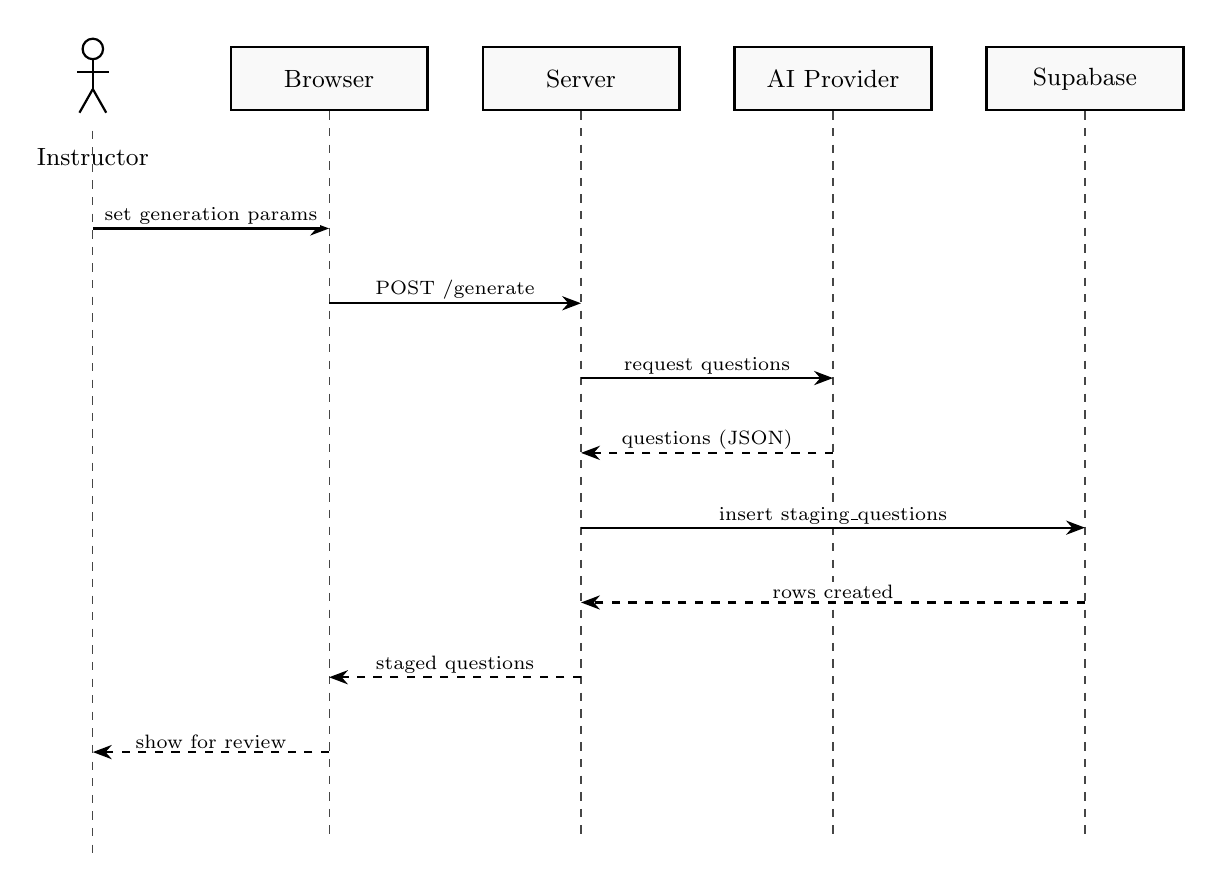
\begin{tikzpicture}

  % --- Lifeline headers (x positions fixed; this is the one diagram
  % type where fixed lanes are the correct, expected layout) ---------
  \node[actorhead] (instructor) at (0,0) {};
  \node[font=\small, below=0.1cm of instructor] {Instructor};

  \node[seqhead] (browser)  at (3.0,0)  {Browser};
  \node[seqhead] (server)   at (6.2,0)  {Server};
  \node[seqhead] (ai)       at (9.4,0)  {AI Provider};
  \node[seqhead] (db)       at (12.6,0) {Supabase};

  \foreach \n in {instructor,browser,server,ai,db}
    \draw[lifeline] (\n.south) -- ++(0,-9.2);

  % --- Messages (fixed vertical step of 0.95cm between rows) --------
  \draw[syncmsg] (0,-1.9) -- node[seqlabel,above]{set generation params} (3.0,-1.9);
  \draw[syncmsg] (3.0,-2.85) -- node[seqlabel,above]{POST /generate} (6.2,-2.85);
  \draw[syncmsg] (6.2,-3.8) -- node[seqlabel,above]{request questions} (9.4,-3.8);
  \draw[retmsg]  (9.4,-4.75) -- node[seqlabel,above]{questions (JSON)} (6.2,-4.75);
  \draw[syncmsg] (6.2,-5.7) -- node[seqlabel,above]{insert staging\_questions} (12.6,-5.7);
  \draw[retmsg]  (12.6,-6.65) -- node[seqlabel,above]{rows created} (6.2,-6.65);
  \draw[retmsg]  (6.2,-7.6) -- node[seqlabel,above]{staged questions} (3.0,-7.6);
  \draw[retmsg]  (3.0,-8.55) -- node[seqlabel,above]{show for review} (0,-8.55);

\end{tikzpicture}

% =====================================================================
% SEQUENCE DIAGRAM 2 -- Compile Paper to PDF (REQ-7.x), with an alt
% fragment covering the REQ-7.3 success/failure split.
% =====================================================================
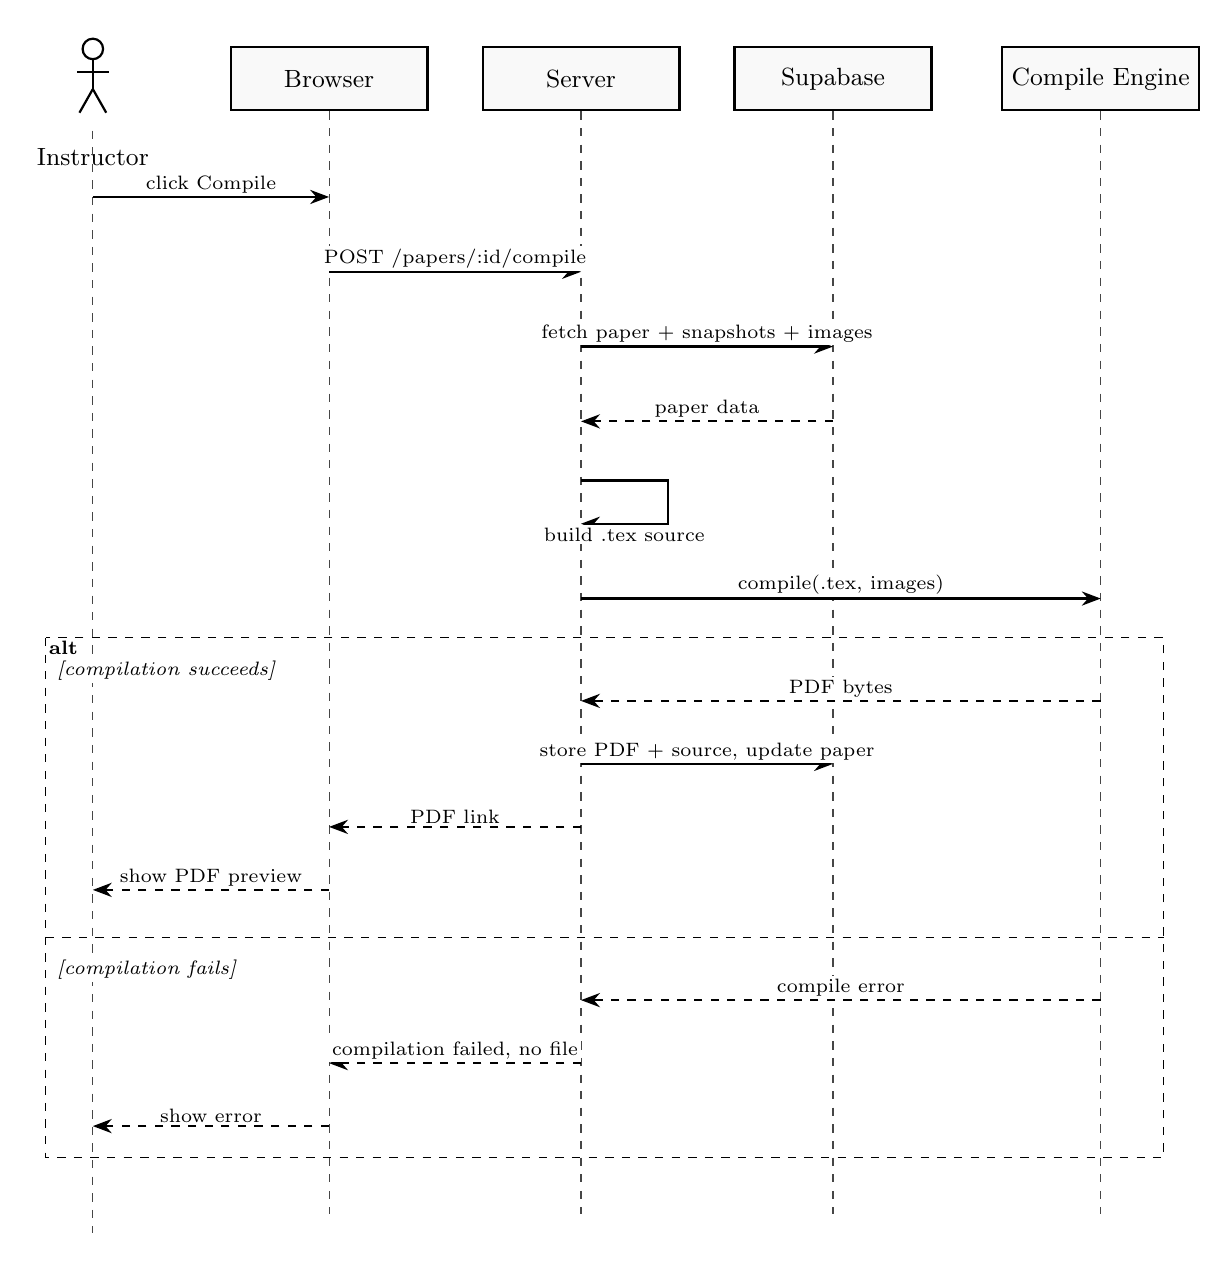
\begin{tikzpicture}

  \node[actorhead] (instructor) at (0,0) {};
  \node[font=\small, below=0.1cm of instructor] {Instructor};

  \node[seqhead] (browser)  at (3.0,0)   {Browser};
  \node[seqhead] (server)   at (6.2,0)   {Server};
  \node[seqhead] (supabase) at (9.4,0)   {Supabase};
  \node[seqhead] (compiler) at (12.8,0)  {Compile Engine};

  \foreach \n in {instructor,browser,server,supabase,compiler}
    \draw[lifeline] (\n.south) -- ++(0,-14.0);

  % --- Preamble: fetch data, build source, invoke compiler ----------
  \draw[syncmsg] (0,-1.5)   -- node[seqlabel,above]{click Compile} (3.0,-1.5);
  \draw[syncmsg] (3.0,-2.45)-- node[seqlabel,above]{POST /papers/:id/compile} (6.2,-2.45);
  \draw[syncmsg] (6.2,-3.4) -- node[seqlabel,above]{fetch paper + snapshots + images} (9.4,-3.4);
  \draw[retmsg]  (9.4,-4.35)-- node[seqlabel,above]{paper data} (6.2,-4.35);

  % self-message: build .tex source
  \draw[syncmsg] (6.2,-5.1) -- ++(1.1,0) -- ++(0,-0.55) -- node[seqlabel,below]{build .tex source} ++(-1.1,0);

  \draw[syncmsg] (6.2,-6.6) -- node[seqlabel,above]{compile(.tex, images)} (12.8,-6.6);

  % --- alt fragment: success / failure -------------------------------
  % Success branch runs all the way to the Instructor (PDF link, then
  % preview shown) so it mirrors the failure branch, which also runs
  % all the way to the Instructor (error shown). Everything on both
  % paths stays inside this one frame -- nothing conditional on the
  % outcome is drawn outside it.
  \draw[dashed] (-0.6,-7.1) rectangle (13.6,-13.7);
  \node[framelabel, anchor=north west] at (-0.6,-7.1) {alt};
  \draw[dashed] (-0.6,-10.9) -- (13.6,-10.9);

  \node[guardlabel, anchor=north west] at (-0.5,-7.35) {[compilation succeeds]};
  \draw[retmsg]  (12.8,-7.9) -- node[seqlabel,above]{PDF bytes} (6.2,-7.9);
  \draw[syncmsg] (6.2,-8.7)  -- node[seqlabel,above]{store PDF + source, update paper} (9.4,-8.7);
  \draw[retmsg]  (6.2,-9.5)  -- node[seqlabel,above]{PDF link} (3.0,-9.5);
  \draw[retmsg]  (3.0,-10.3) -- node[seqlabel,above]{show PDF preview} (0,-10.3);

  \node[guardlabel, anchor=north west] at (-0.5,-11.15) {[compilation fails]};
  \draw[retmsg]  (12.8,-11.7) -- node[seqlabel,above]{compile error} (6.2,-11.7);
  \draw[retmsg]  (6.2,-12.5)  -- node[seqlabel,above]{compilation failed, no file} (3.0,-12.5);
  \draw[retmsg]  (3.0,-13.3)  -- node[seqlabel,above]{show error} (0,-13.3);

\end{tikzpicture}

% =====================================================================
% ACTIVITY DIAGRAM 1 -- Question Intake & Staging Workflow
% (REQ-3.x Multimodal Extraction, REQ-4.x Staging Sandbox)
% =====================================================================
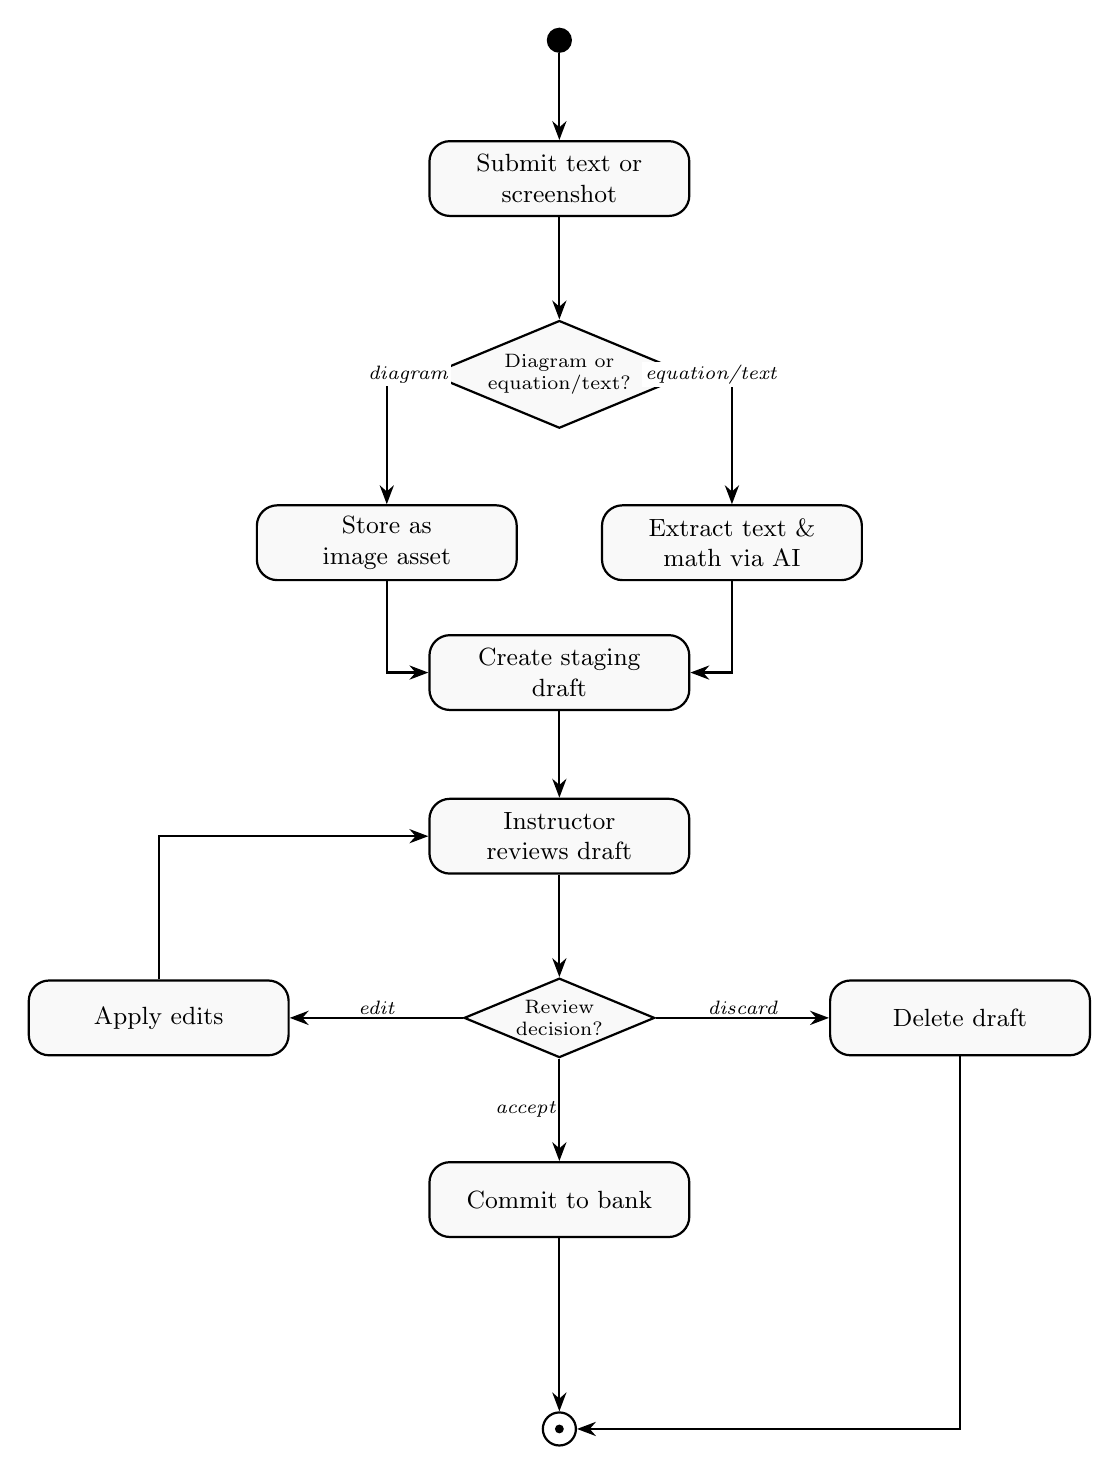
\begin{tikzpicture}[node distance=1.1cm and 1.6cm]

  \node[actstart] (start) {};
  \node[actaction, below=of start] (submit) {Submit text or\\screenshot};
  \node[actdecision, below=1.3cm of submit] (typedec) {Diagram or\\equation/text?};

  \node[actaction, below left=1.3cm and -0.3cm of typedec] (storeimg) {Store as\\image asset};
  \node[actaction, below right=1.3cm and -0.3cm of typedec] (extract) {Extract text \&\\math via AI};

  \node[actaction, below=2.6cm of typedec] (stage) {Create staging\\draft};
  \node[actaction, below=of stage] (reviewnode) {Instructor\\reviews draft};
  \node[actdecision, below=1.3cm of reviewnode] (revdec) {Review\\decision?};

  \node[actaction, left=2.2cm of revdec] (editnode) {Apply edits};
  \node[actaction, below=1.3cm of revdec] (commit) {Commit to bank};
  \node[actaction, right=2.2cm of revdec] (discard) {Delete draft};

  \node[actend, below=2.2cm of commit] (end) {};
  \fill (end) circle (1.6pt);

  \draw[actflow] (start) -- (submit);
  \draw[actflow] (submit) -- (typedec);
  \draw[actflow] (typedec) -| node[actlabel, pos=0.25]{diagram} (storeimg);
  \draw[actflow] (typedec) -| node[actlabel, pos=0.25]{equation/text} (extract);
  \draw[actflow] (storeimg) |- (stage);
  \draw[actflow] (extract)  |- (stage);
  \draw[actflow] (stage) -- (reviewnode);
  \draw[actflow] (reviewnode) -- (revdec);
  \draw[actflow] (revdec) -- node[actlabel, above]{edit} (editnode);
  \draw[actflow] (editnode) |- (reviewnode);
  \draw[actflow] (revdec) -- node[actlabel, left]{accept} (commit);
  \draw[actflow] (revdec) -- node[actlabel, above]{discard} (discard);
  \draw[actflow] (commit) -- (end);
  \draw[actflow] (discard) |- (end);

\end{tikzpicture}

% =====================================================================
% ACTIVITY DIAGRAM 2 -- Paper Assembly & Compilation Workflow
% (REQ-6.x Blueprint Generator, REQ-7.x Document Compilation)
% =====================================================================
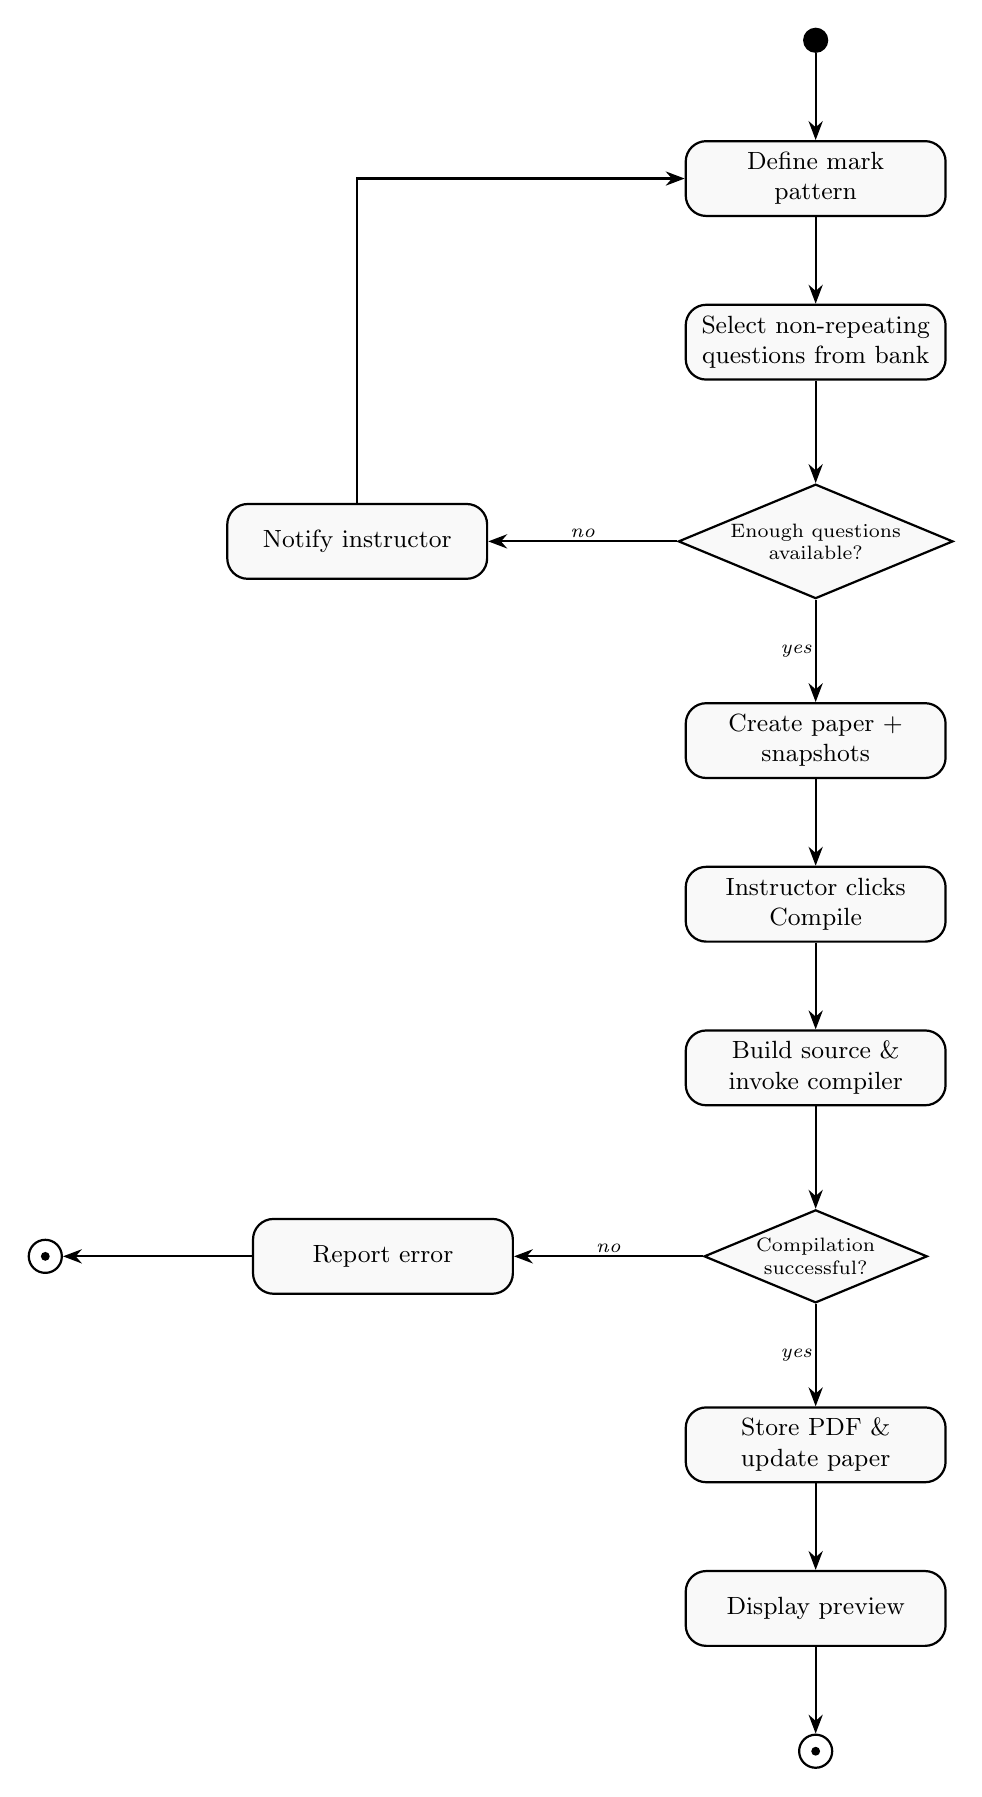
\begin{tikzpicture}[node distance=1.1cm and 1.6cm]

  \node[actstart] (start) {};
  \node[actaction, below=of start] (pattern) {Define mark\\pattern};
  \node[actaction, below=of pattern] (select) {Select non-repeating\\questions from bank};
  \node[actdecision, below=1.3cm of select] (enoughdec) {Enough questions\\available?};

  \node[actaction, left=2.4cm of enoughdec] (notify) {Notify instructor};
  \node[actaction, below=1.3cm of enoughdec] (createpaper) {Create paper +\\snapshots};
  \node[actaction, below=of createpaper] (clickcompile) {Instructor clicks\\Compile};
  \node[actaction, below=of clickcompile] (buildinvoke) {Build source \&\\invoke compiler};
  \node[actdecision, below=1.3cm of buildinvoke] (successdec) {Compilation\\successful?};

  \node[actaction, left=2.4cm of successdec] (reporterr) {Report error};
  \node[actaction, below=1.3cm of successdec] (storepdf) {Store PDF \&\\update paper};
  \node[actaction, below=of storepdf] (preview) {Display preview};

  \node[actend, left=2.4cm of reporterr] (endfail) {};
  \fill (endfail) circle (1.6pt);
  \node[actend, below=of preview] (endok) {};
  \fill (endok) circle (1.6pt);

  \draw[actflow] (start) -- (pattern);
  \draw[actflow] (pattern) -- (select);
  \draw[actflow] (select) -- (enoughdec);
  \draw[actflow] (enoughdec) -- node[actlabel, above]{no} (notify);
  \draw[actflow] (notify) |- (pattern);
  \draw[actflow] (enoughdec) -- node[actlabel, left]{yes} (createpaper);
  \draw[actflow] (createpaper) -- (clickcompile);
  \draw[actflow] (clickcompile) -- (buildinvoke);
  \draw[actflow] (buildinvoke) -- (successdec);
  \draw[actflow] (successdec) -- node[actlabel, above]{no} (reporterr);
  \draw[actflow] (reporterr) -- (endfail);
  \draw[actflow] (successdec) -- node[actlabel, left]{yes} (storepdf);
  \draw[actflow] (storepdf) -- (preview);
  \draw[actflow] (preview) -- (endok);

\end{tikzpicture}

\end{document}
